%%%%%%%%%%%%%%%%%%%%%%%%%%%%%%%% 
\section{The 35-t Prototype} 
\label{sec:proto-35t}

The 35-t prototype first phase of operations (Phase-1) was designed
to demonstrate that a non-evacuable membrane cryostat could satisfy
the DUNE FD requirement that oxygen contamination of the liquid argon
be less than 200 parts per trillion (ppt), and that such a cryostat
could stably maintain that level.  The construction and operation of
the 35-t cryostat provided an opportunity to address a wide variety
challenges that the far detector will face.  These included
procurement of materials and services, construction procedures and
development of operational procedures to ensure safety and the ability
of the cryostat to maintain high-purity liquid argon.  Phase-1 of the
35-t prototype was successfully completed in 2014.

The second phase of 35-t prototype operations (Phase-2) includes the
installation and operation a small-scale, single-phase LArTPC and
photon detector in the cryostat.  This phase will focus on the
performance of active detector elements, which will employ many of the
novel features of the DUNE single-phase FD design.  Phase-2 is
currently under construction and plans to take data in summer
2015.

\subsection{35-t Phase-1: Cryostat Construction}

The LBNE project contracted with the Japanese company IHI
to build the 35-t cryostat at Fermilab's PC-4 facility.
Since this is also where the Liquid Argon Purity Demonstrator (LAPD)\cite{bib:lapdP07005}
was built, a large portion of the cryogenic-process 
equipment installed for LAPD could be re-used for the 35-t.
The proximity and size (30-t) of LAPD also offers the possibility using LAPD as 
a partial storage vessel for LAr if the 35-t ever needs to be emptied.

The 35-t employs a submersible pump to circulate the LAr from the
cryostat to the filters.  Two pumps were installed for redundancy, but
only one is used at a time.  Figure~\ref{fig:35cutaway} shows a
cutaway view of the cryostat and a photograph of the interior of the
completed cryostat.
\begin{cdrfigure}[Cutaway view]{35cutaway}{(left) Cutaway view of the 35-t cryostat. (right) Interior
photograph of the completed cryostat.}
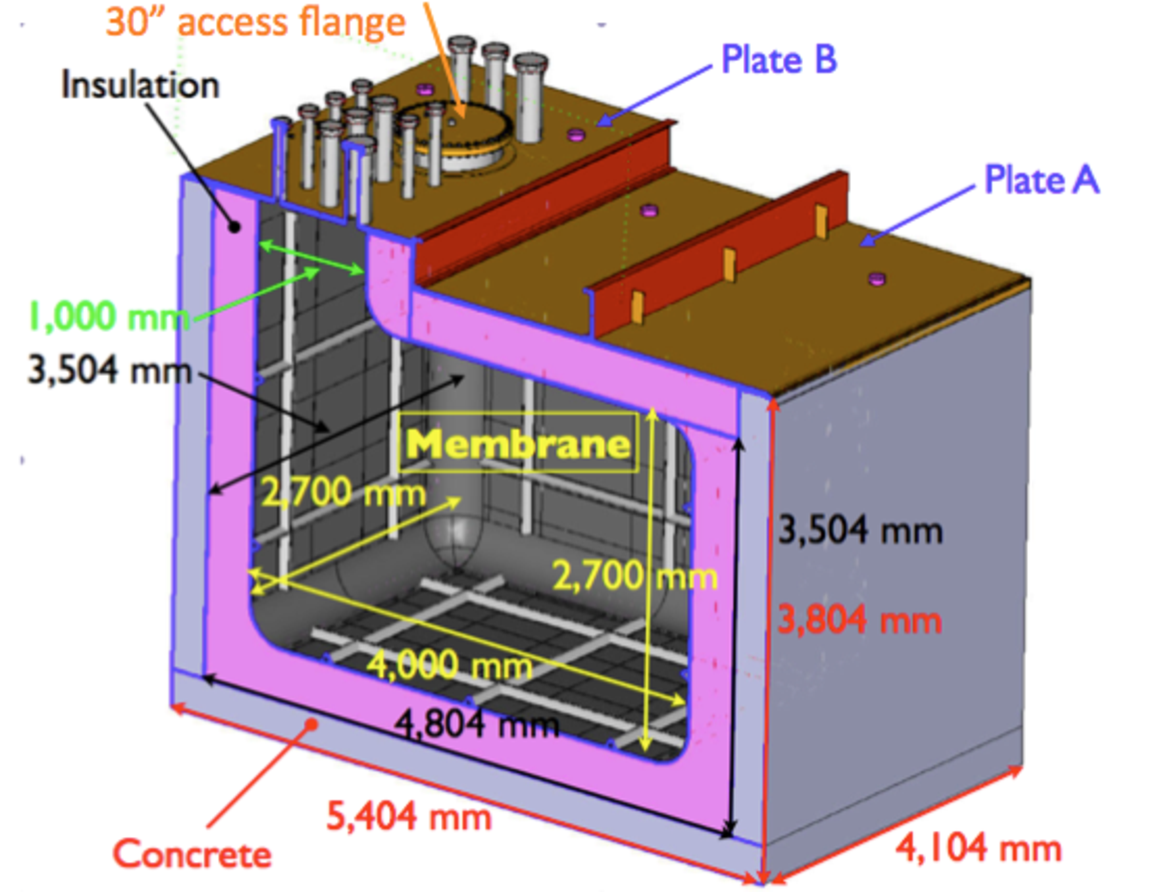
\includegraphics[width=0.60\textwidth]{35TCutaway}
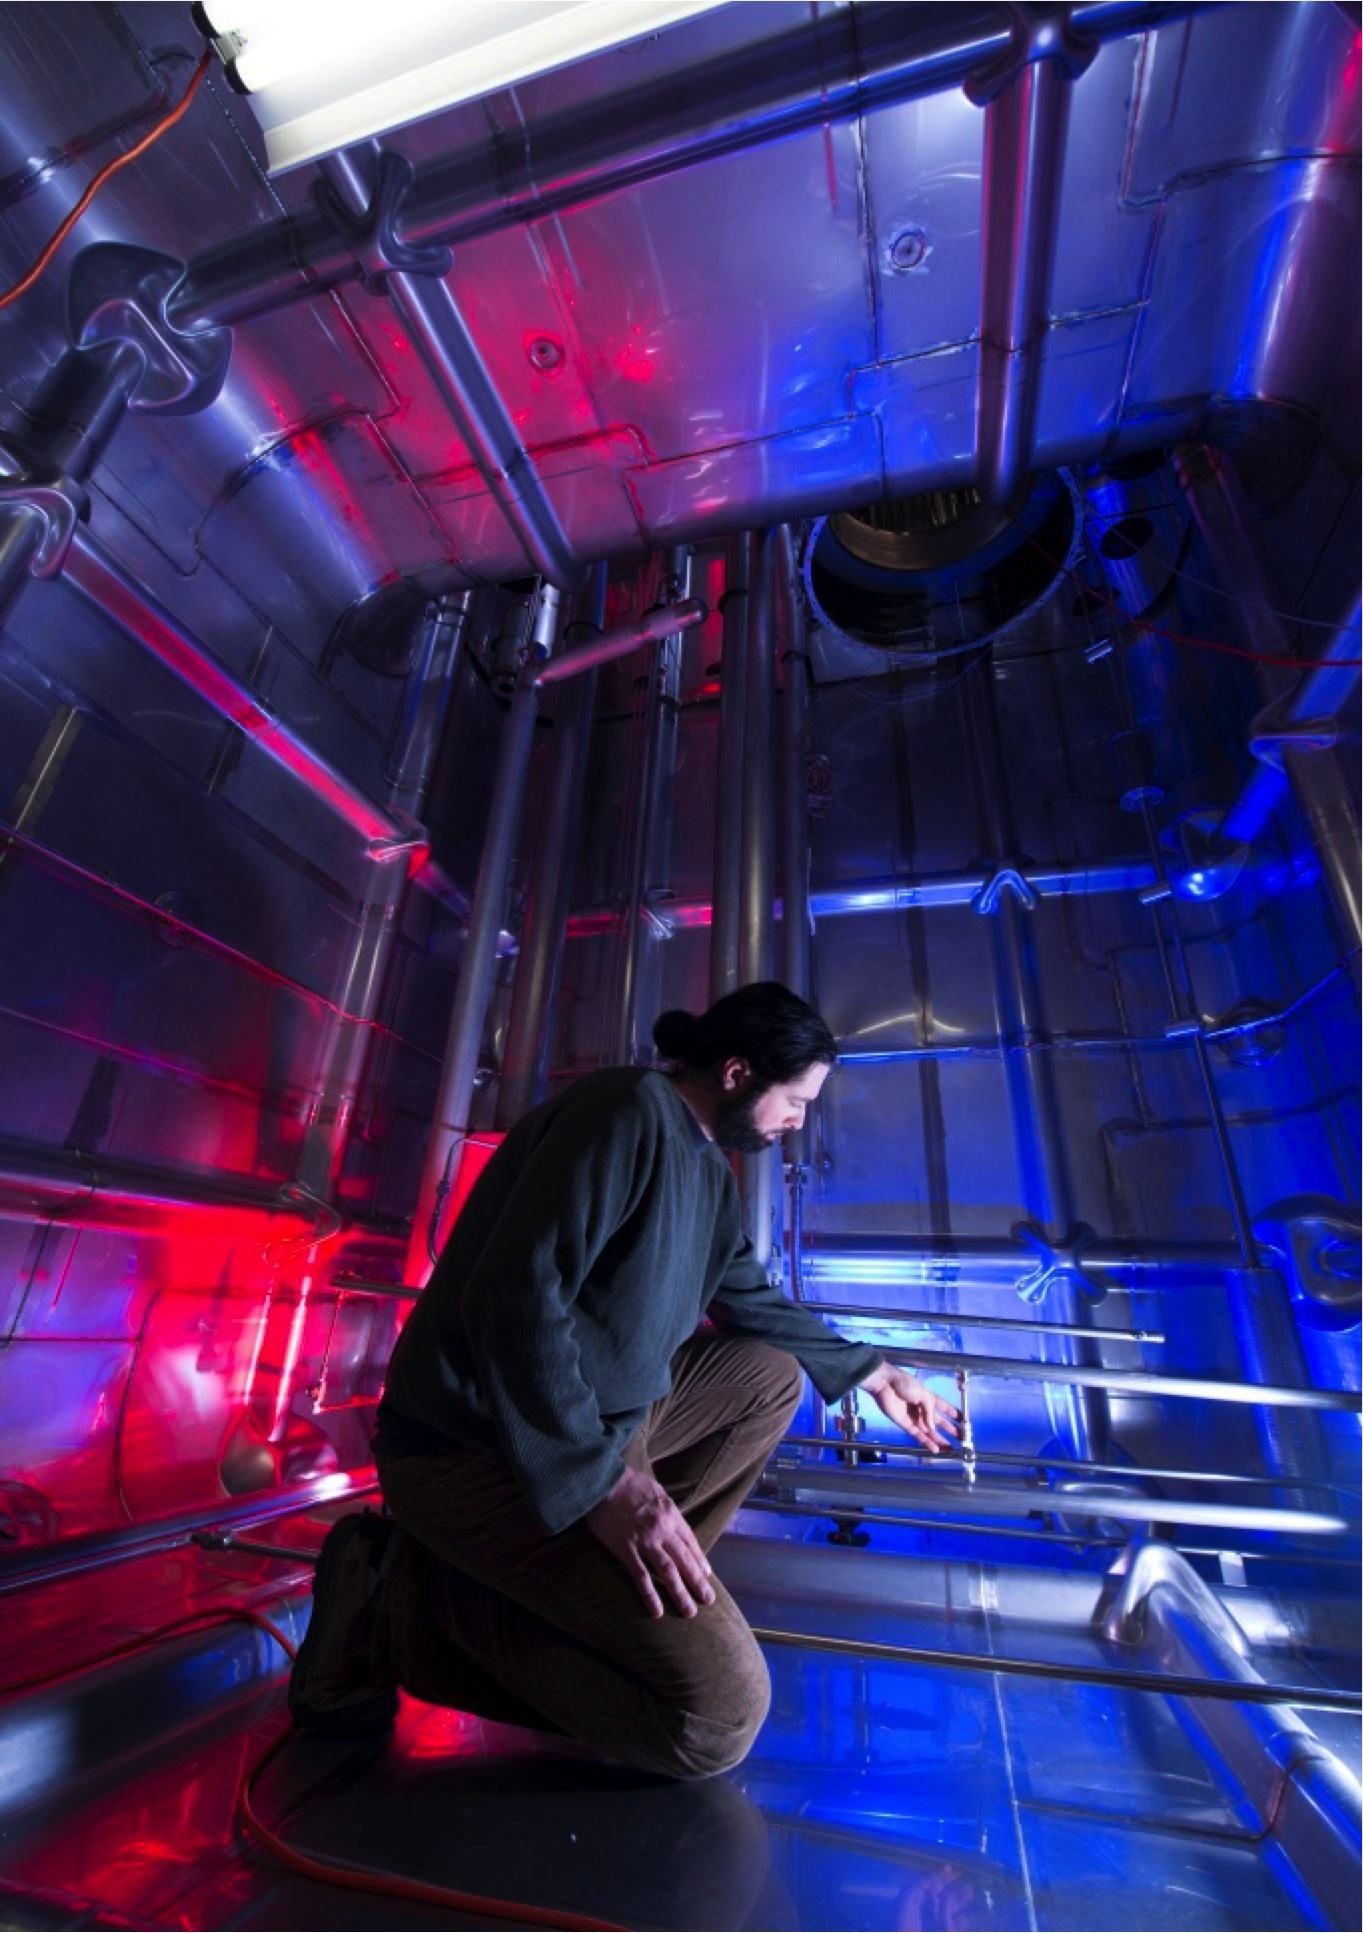
\includegraphics[width=0.35\textwidth]{35TCryo}
\end{cdrfigure}
Table~\ref{tab:35Tdimensions} gives the details of the construction
materials and the dimensions for the 35-t.  
\begin{cdrtable}[35-t Details and Dimensions]{ll}{35Tdimensions}
{35-t Details and Dimensions}
Parameter & Value \\ \toprowrule
Cryostat Volume	&      29.16 m3\\ \colhline
Liquid Argon total mass	 &     38.6 metric t       \\ \colhline
Inner dimensions	&      4.0 m (L) x 2.7 m (W) x 2.7 m (H)\\ \colhline
Outer dimensions        &      5.4 m (L) x 4.1 m (W) x 4.1 m (H)\\ \colhline
Membrane		&      2.0 mm thick corrugated 304 SS\\ \colhline
Insulation		&      0.4 m polyurethane foam\\ \colhline
Secondary barrier system	   &   0.1 mm thick fiberglass\\ \colhline
Vapor barrier	Normal	  &    1.2 mm thick carbon steel\\ \colhline
Steel reinforced concrete	    &  0.3 m thick layer\\ 
\end{cdrtable}
More information can be found in\cite{bib:membcryo1573}.  The
insulation thickness is 0.4~m rather than the 1.0~m chosen for the
reference design, but the heat load in the small-scale cryostat was
still manageable.  The techniques of membrane-cryostat construction
were demonstrated to be adequate for high-purity LAr operation.
Welding of corrugated panels, removal of leak-checking dye penetrant
or ammonia-activated leak-detecting paints, and
post-construction-cleaning methods were tested and found to be
suitable.


\subsection{35-t Phase-1: Operation and Performance} 
Once construction was completed, the argon filling of the cryostat
commenced.  In the first stage, gaseous Ar was used to purge the
cryostat and begin the removal of impurities.  As previously
demonstrated by LAPD, this ``Piston Purge'', can efficiently remove
much of the gaseous impurities.  The next stage involves circulating
the gas while filtering, which removes residual water and oxygen, but
not nitrogen.  Figure~\ref{fig:35TPurge} graphically shows the
room-temperature, gas-phase purification process.  
\begin{cdrfigure}[Gas Ar Purge and Recirculation]{35TPurge}
{Gas phase of removing impurities in the 35-t. These quantities are 
being measured by various gas analyzers. The first stage of the 
purification is a process called the ``Piston Purge''.  The second 
stage is ``Recirculation with Filtering''. The gap between the two 
steps was due to troubleshooting a leak.}
  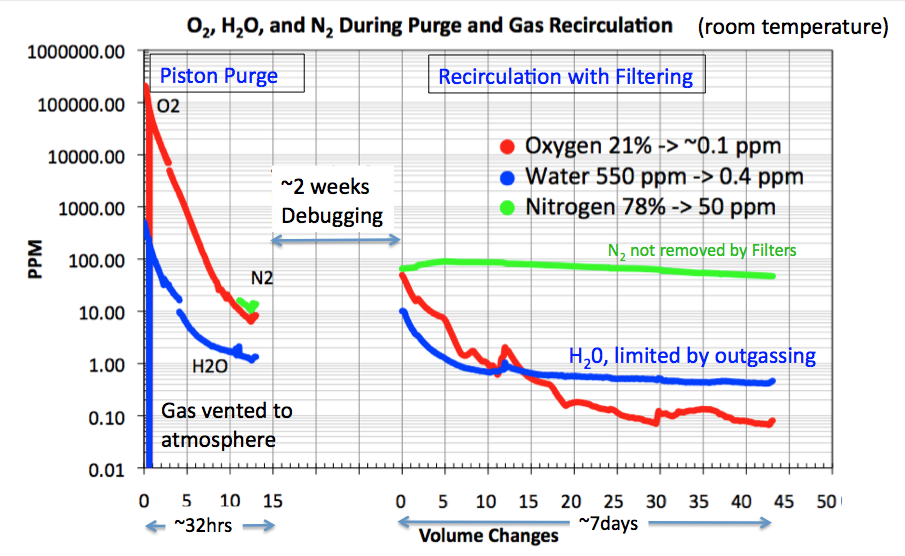
\includegraphics[width=0.8\textwidth]{35TPurgeAndRecirc}
\end{cdrfigure}
The initial state, $t=0$, reflects the initial values for oxygen,
water and nitrogen in the ``dry air'' state.  These measurements are
made by a variety of monitors that sample the gas in the cryostat.


Once room-temperature, gas-phase filtering was no longer improving
purity, the cooldown and LAr fill stage began.  A gas/liquid spray
method was used to cool down the cryostat.  This generated a turbulent
mixing of cold gas in the cryostat and cools the entire surface.  The
cooldown rate was approximately 7$^\circ$K/hr and was maintained below
than the maximum specified by the manufacturer (about 12$^\circ$K/hr).
Once the cooldown was complete, the LAr was transferred into the
cryostat and recirculating purification begun.

During liquid recirculation and purification, dedicated
purity monitors were used to measure electron lifetime, which can 
be translated into equivalent oxygen contamination levels.
Figure~\ref{fig:35TElectronLifetime} shows the electron lifetime from the start of the
LAr Pump operation until the end of the Phase-1 run. 
\begin{cdrfigure}[35t Electron Lifetime]{35TElectronLifetime}{LAr electron lifetmes as measured by 
Cryostat Purity Monitors. Significant events are annotated on the plot. Major divisions on horizontal axis 
are one week periods. Equivalent purity levels are shown as dashed horizontal lines.}
  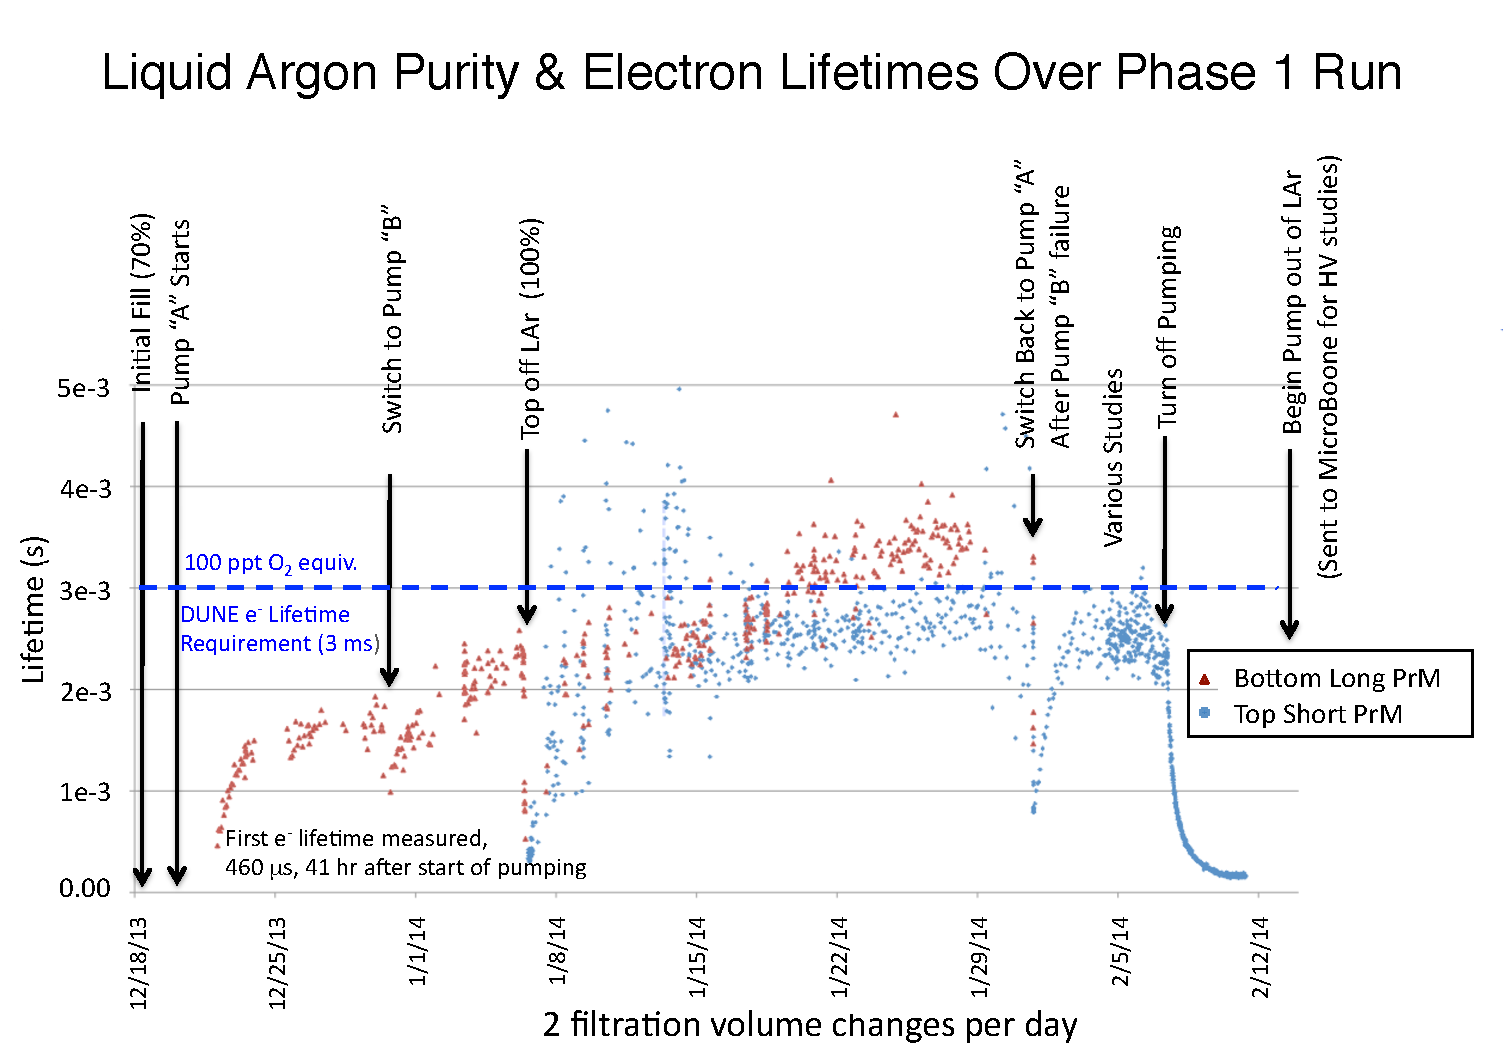
\includegraphics[width=0.7\textwidth]{LifetimePlotBigger.pdf}
\end{cdrfigure}
In general, the electron lifetime improved as a function of pump 
on-time, but there were several incidents that spoiled the lifetime.
Electron lifetimes of $>$1.4~ms were consistently achieved.


\subsection{35-t Phase-1: Conclusions}
The 35-t Phase-1 run successfully demonstrated that there is nothing innate to
membrane cryostat technology that would prohibit achieving the stated goals of the
DUNE Far Detector. In addition, experience gained in operating the 35-t system
will inform future design decisions, e.g., the loss of purity when switching pumps is
undesireable, and can likely be avoided by improved system design. Future system
designs could also avoid coupling acoustical vibrations into the cryostat by choosing
to locate the pumps externally, which would have the added benefit of facilitating
maintenance and repair.

\subsection{35-t Phase-2: Installation of Active Detectors}
Phase-2 of the the 35-t prototype extends the scope to include a
fully operational TPC and photon detector in the previously built
cryostat.  After detector installation, the prototype will be filled
with liquid argon and operated for a several-month-long cosmic ray
run.  External plastic scintillator paddles placed around the cryostat
will be used to produce trigger signals as well as rough position
measurements of the incoming cosmic rays.  Commissioning is expected
to begin in August 2015.  Figure~\ref{fig:35TTPC} shows a model of the
TPC inside the cryostat and a trial assembly of the TPC outside of the
cyrostat.

\begin{cdrfigure}[35-t with TPC]{35TTPC}{(left) Rendering of the
35-t Cryostat with TPC and photon detectors installed. 
Note the position of the APA, which is asymmetrically located and 
splits the volume into two separate drift regions.
The length of the longer one of these is close to what is proposed for the far detector. 
The other has a shorter drift length due to lack of space.
(right) A trial assembly of the TPC.
}
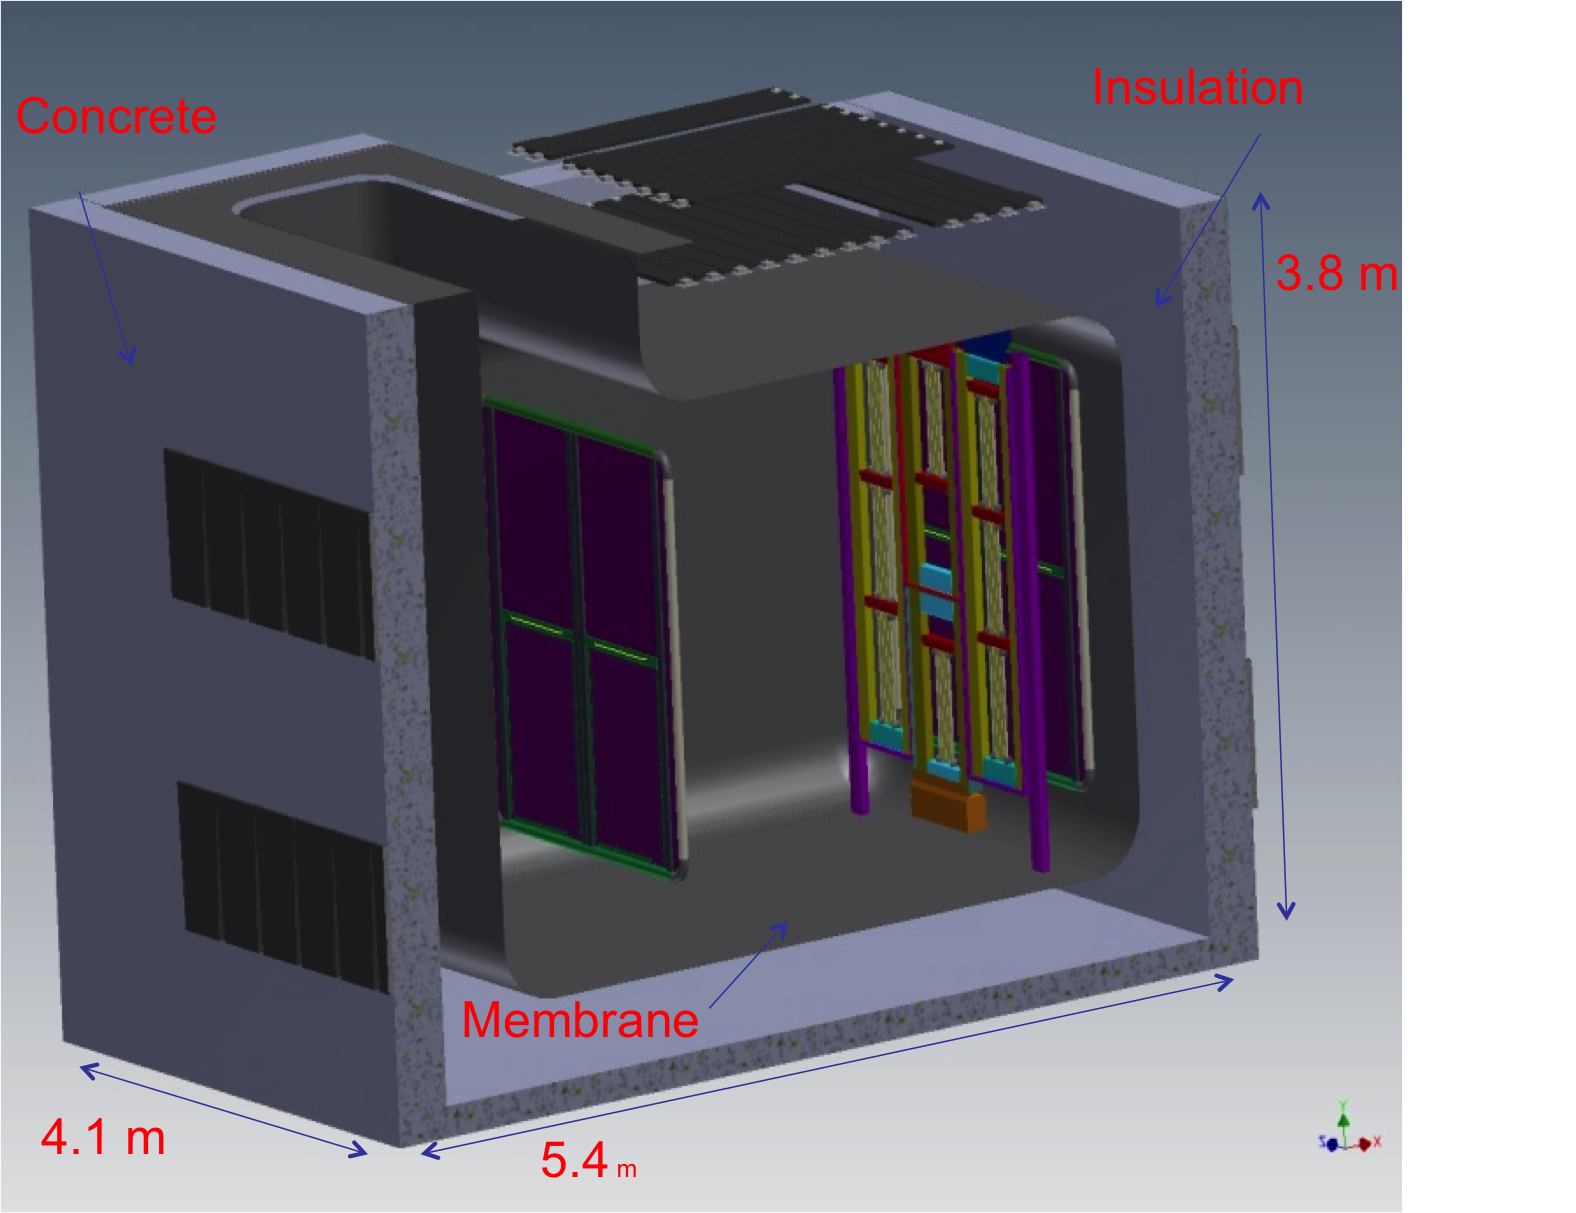
\includegraphics[width=0.55\textwidth]{35TTPC}  
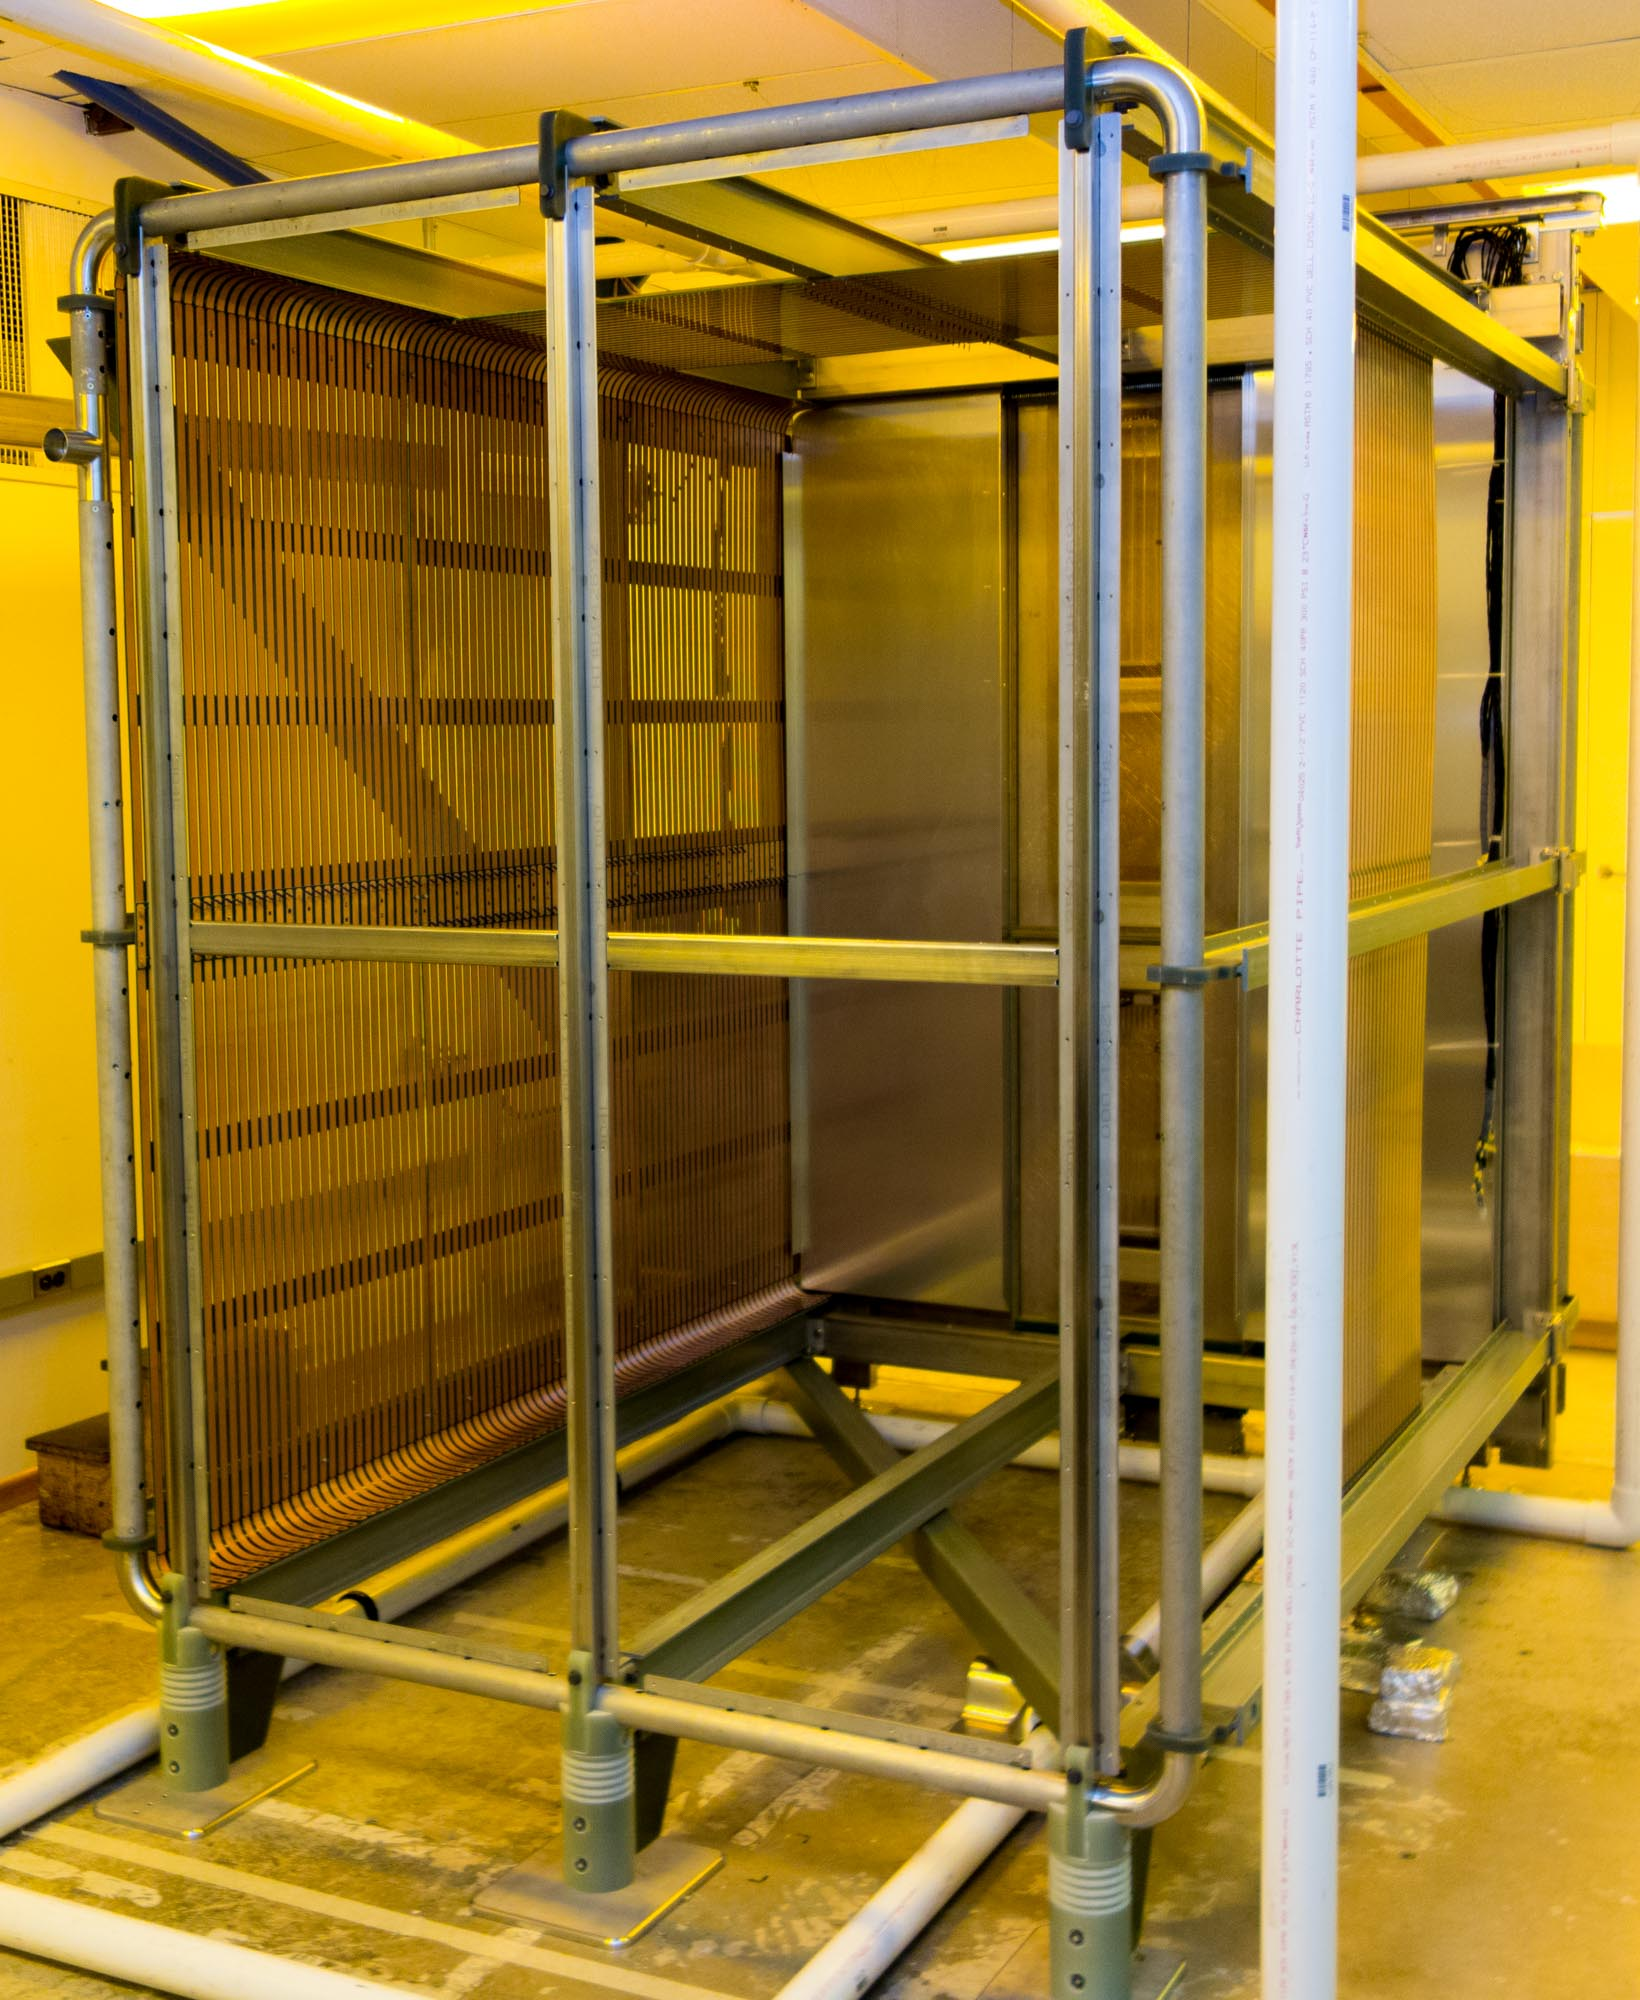
\includegraphics[width=0.35\textwidth]{35TTrial}  
\end{cdrfigure}

The Phase-2 prototype incorporates many of the design elements described in previous
sections of this document.
In many cases, these include novel features that have never previously been tested
in an operational TPC.
Rather than reiterate them all here, some of the more important
aspects are collected in Table~\ref{tab:35TDesign}.

\begin{cdrtable}[35-t Design Elements]{lcl}{35TDesign}{35-t Design Elements}
 Design Aspect& Section & How Tested\\ \toprowrule
Modular APAs with wrapped wires & \ref{subsec:fd-ref-apa}&Build small-scale APA Modules with FD design\\
\colhline
Vertical Gaps between APAs &\ref{sec:detectors-fd-ref-tpc}& Assemble APAs side-by-side.\\
&&Study reco'd tracks that cross the gaps.\\
\colhline
Horizontal Gaps between APAs &\ref{sec:detectors-fd-ref-tpc}& Build two shorter APAs and stack vertically\\
&&Study reco'd tracks that cross the gaps\\
\colhline
Field cage constructed of &\ref{sec:detectors-fd-ref-tpc}&Operate at HV 
and measure field uniformity\\
FR4 Printed Circuit Board \\
\colhline
APAs immersed in active volume &\ref{sec:detectors-fd-ref-tpc}& Study reco'd tracks that cross APAs\\
\colhline
Cold Digital Electronics & \ref{sec:detectors-fd-ref-ce} & Measure noise performance etc. {\it in situ}\\
\colhline
Waveguide-style Photon Detector& \ref{sec:detectors-fd-ref-pd}&Install in APAs. Measure lightyield\\
\colhline
Triggerless-capable DAQ & \ref{sec:detectors-fd-ref-daq} & Take data using multiple DAQ modes\\ 
\end{cdrtable}

\subsection{35-t Phase-2: Simulation, Reconstruction and Analysis}
The performance of many of the DUNE design elements discussed in
Table~\ref{tab:35TDesign} will be studied with data collected in 2015.
Study of these design features requires simulation, reconstruction and
analysis of 35-t data.  This will be done with the help of the
LarSoft package, which is also used to simulate and reconstruct data
from the ArgoNeuT and MicroBoone experiments.  Reuse of software
developed for those experiments can greatly facilitate 35-t
development.  However, the novel hardware features of the 35t
prototype necessitate new software developments as well.  Among the
required new software developments are:
\begin{itemize}
\item{Code to divide the wrapped wires into as many as five individual linear segments. 
A hit on a single electronic channel can, in principle, be related to a
signal on any of these segments.}
\item{``Disambiguation'' code to identify which of the possible wire segments was actually responsible
for the observed hit}
\item{Code for determining the start time of the event ($t_0$). Since the 35-t prototype DAQ can
run ``triggerless,'' methods are needed for finding the $t_0$ in data. Information from the external 
scintillator paddles as well as the internal photon detectors can be used.}
\item{Code for ``stitching'' together track segments observed in different tracking volumes. 
Since hits can come from either side of the four APAs, there are 
effectively eight separate tracking volumes, 
which are treated as separate TPCs.}
\end{itemize}

With these simulation and reconstruction tools in hand, ``physics''
analysis of the data can be undertaken.
In addition to the analyses needed to validate the new detector design elements, there are also
some analyses of basic LArTPC performance that are needed as well.
Among the highest priority analysis tasks are:

\begin{itemize}
\item{Basic detector performance: signal/noise, purity measured with tracks, track direction resolution, 
photon detector light yield}
\item{Measurement of distortions due to space charge and field non-uniformity}
\item{Measurements of different types of particles: muons, protons, neutrons, pions}
\end{itemize}

The results obtained by operating the 35-t Phase-2 prototype and the analysis of its data are expected
to be very valuable in defining the final far detector design. 
